\documentclass{article}

\usepackage{ctex}
\usepackage[top=0.7in,bottom=0.7in,left=0.5in,right=0.5in]{geometry}
\usepackage{array}
\usepackage{multirow}
\usepackage{graphicx}
\usepackage{fancyhdr}
\usepackage{lastpage}
\usepackage{extramarks}
\usepackage{amsmath}
\usepackage{listings}
\usepackage{fontspec}
\newfontfamily\menlo{Menlo}
\usepackage{xcolor} % 定制颜色
\definecolor{mygreen}{rgb}{0,0.6,0}
\definecolor{mygray}{rgb}{0.5,0.5,0.5}
\definecolor{mymauve}{rgb}{0.58,0,0.82}
\lstset{ %
backgroundcolor=\color{white},      % choose the background color
basicstyle=\footnotesize\ttfamily,  % size of fonts used for the code
columns=fullflexible,
tabsize=4,
breaklines=true,               % automatic line breaking only at whitespace
captionpos=b,                  % sets the caption-position to bottom
commentstyle=\color{mygreen},  % comment style
escapeinside={\%*}{*)},        % if you want to add LaTeX within your code
keywordstyle=\color{blue},     % keyword style
stringstyle=\color{mymauve}\ttfamily,  % string literal style
frame=single,
rulesepcolor=\color{red!20!green!20!blue!20},
% identifierstyle=\color{red},
language=c++,
}

\newcommand{\hmwkTitle}{加里森的任务\ 实验报告}
\newcommand{\hmwkClass}{数据结构}
\newcommand{\hmwkClassInstructor}{}
\newcommand{\hmwkAuthorName}{毛子恒\ 李臻\ 张梓靖}

\pagestyle{fancy}
\lhead{\hmwkAuthorName}
\chead{\hmwkClass\ : \hmwkTitle}
\rhead{\firstxmark}
\lfoot{\lastxmark}
\cfoot{\thepage}
\renewcommand\headrulewidth{0.4pt}
\renewcommand\footrulewidth{0.4pt}

\title{\hmwkClass\ :\hmwkTitle}
\author{\hmwkAuthorName}

\setcounter{tocdepth}{1}

\begin{document}

\maketitle  

\section*{小组成员}

\setlength{\tabcolsep}{9mm}
{
    \begin{table}[htbp]
        \centering
        \begin{tabular}{llll}
            班级:2019211309 & 姓名:毛子恒 & 学号:2019211397 & 分工:代码\ 文档   \\
            
            班级:2019211310 & 姓名:李臻   & 学号:2019211458 & 分工:测试\ 文档   \\
            
            班级:2019211308 & 姓名:张梓靖 & 学号:2019211379 & 分工:可视化\ 文档 \\
        \end{tabular}
    \end{table}
}

\tableofcontents
\newpage

\section{需求分析}

\subsection{题目描述}

在由序号为$1$至$n$的$n$个元素依次排列并且首尾相接而组成的环中,规定初始时从序号$1$开始依次经过$2,3,...$元素走到第$n$个元素的方向为正方向。

初始时以第$x$个元素为起点$st$,重复以下过程$n-1$次:以$st$为第1个元素,沿正方向找到第$y$个元素$del$,从环中删除$del$元素,再将原$del$的下一个元素作为新的$st$。

求经过$n-1$次操作之后,环中仅剩的一个元素的序号是否是1。

\subsection{输入描述}

程序从标准输入中读入数据。输入一行三个整数,用空格分隔,分别表示$n,x,y$。

其中各个值的范围需要满足$1 < n \leq 10^4\quad 0 < x \leq n\quad 0 < y \leq 5\times 10^4$。

\subsection{输出描述}

程序向标准输出中输出结果。

输出分为三种情况:

\begin{enumerate}
    \item 输入合法,程序正常运行结束。此时输出两行,第一行一个字符串"Yes"或者"No"(不带引号),分别表示最后一个元素是/不是1,第二行一个数字,表示最后一个元素的序号。
    \item 输入不合法。此时输出一行一个字符串"Please check your input."(不带引号)。
    \item 程序发生运行时错误,比如内存分配失败。此时程序没有输出。
\end{enumerate}

\subsection{样例输入输出}

\subsubsection{样例输入输出1}

【输入】

\begin{lstlisting}[language={bash},
    basicstyle=\small\menlo]
10 1 3
\end{lstlisting}

【输出】

\begin{lstlisting}[language={bash},
    basicstyle=\small\menlo]
No
4
\end{lstlisting}

\subsubsection{样例输入输出2}

【输入】

\begin{lstlisting}[language={bash},
    basicstyle=\small\menlo]
10 3 7
\end{lstlisting}

【输出】

\begin{lstlisting}[language={bash},
    basicstyle=\small\menlo]
Yes
1
\end{lstlisting}

\subsubsection{样例输入输出3}

【输入】

\begin{lstlisting}[language={bash},
    basicstyle=\small\menlo]
100 87 305
\end{lstlisting}

【输出】

\begin{lstlisting}[language={bash},
    basicstyle=\small\menlo]
No
50
\end{lstlisting}

\subsubsection{样例输入输出4}

【输入】

\begin{lstlisting}[language={bash},
    basicstyle=\small\menlo]
1000 725 801
\end{lstlisting}

【输出】

\begin{lstlisting}[language={bash},
    basicstyle=\small\menlo]
No
798
\end{lstlisting}

\subsubsection{样例输入输出5}

【输入】

\begin{lstlisting}[language={bash},
    basicstyle=\small\menlo]
1 1 3
\end{lstlisting}

【输出】

\begin{lstlisting}[language={bash},
    basicstyle=\small\menlo]
Please check your input.
\end{lstlisting}

\subsubsection{样例输入输出6}

【输入】

\begin{lstlisting}[language={bash},
    basicstyle=\small\menlo]
5 6 3
\end{lstlisting}

【输出】

\begin{lstlisting}[language={bash},
    basicstyle=\small\menlo]
Please check your input.
\end{lstlisting}

\subsection{程序功能}

程序通过给定的$n,x,y$计算出最后环中仅剩的元素序号,并且与1比较。

\section{概要设计}

\subsection{问题解决的思路}

使用单循环链表维护此约瑟夫环,首先在链表中依次插入$n$个结点表示$n$名队员,以$now$指针模拟计数过程。

从头结点找到第$x$个结点,此后执行以下操作$n-1$次:找到当前结点之后的第$y-1$个结点,删除这个结点。

此题中单循环链表实现了初始化、判空、在指定位置增加节点、删除指定位置的节点、释放空间这五种操作。

\subsection{链表的定义}

\begin{lstlisting}[language={C},
    numbers=left,
    numberstyle=\tiny\menlo,
    basicstyle=\small\menlo]
// 数据对象
typedef struct node
{
    int item;
    struct Node * next;
} Node;

typedef Node * List;

// 基本操作
/*
 * 操作:初始化链表
 * 后件:plist指向一个循环链表的头结点
 */
void initList(List * plist);

/*
 * 操作:判断链表是否为空
 * 前件:list是循环链表的头结点
 * 后件:如果该链表为空,返回true,否则返回false
 */
bool isEmpty(const List list);

/*
 * 操作:向链表的某个节点后插入一个节点
 * 前件:pnode是链表中的某一个节点
 * 后件:如果成功,pnode之后添加一个新节点,item属性为传入的第二个参数
 */
void addNode(List pnode, int item);

/*
 * 操作:删除链表中指定的节点
 * 前件:pnode是需要删除的节点的前驱且不是头结点
 * 后件:删除链表中的pnode节点的后继
 */
void delNode(List pnode);

/*
 * 操作:找到链表中某一节点的后继
 * 前件:pnode指向链表中的某一个节点
 * 后件:函数返回pnode的后继,并且跳过头结点
 */
List nextNode(const List pnode);

/*
 * 操作:释放链表空间
 * 前件:plist指向需要释放空间的链表的头结点
 * 后件:释放plist指向链表的空间,plist重置为空指针
 */
void destroyList(List * plist);
\end{lstlisting}

\subsection{主程序的流程}

\begin{enumerate}
    \item 输入
    \item 初始化链表
    \item 在链表中依次插入$n$个结点
    \item 找到第$x$个结点
    \item 循环$n-1$次:找到当前节点之后的第$y-1$个结点,删除这个结点
    \item 输出
    \item 释放空间
\end{enumerate}

\subsection{各程序模块之间的层次关系}

函数调用关系图如图1。

\begin{figure}[htbp]
    
    \centering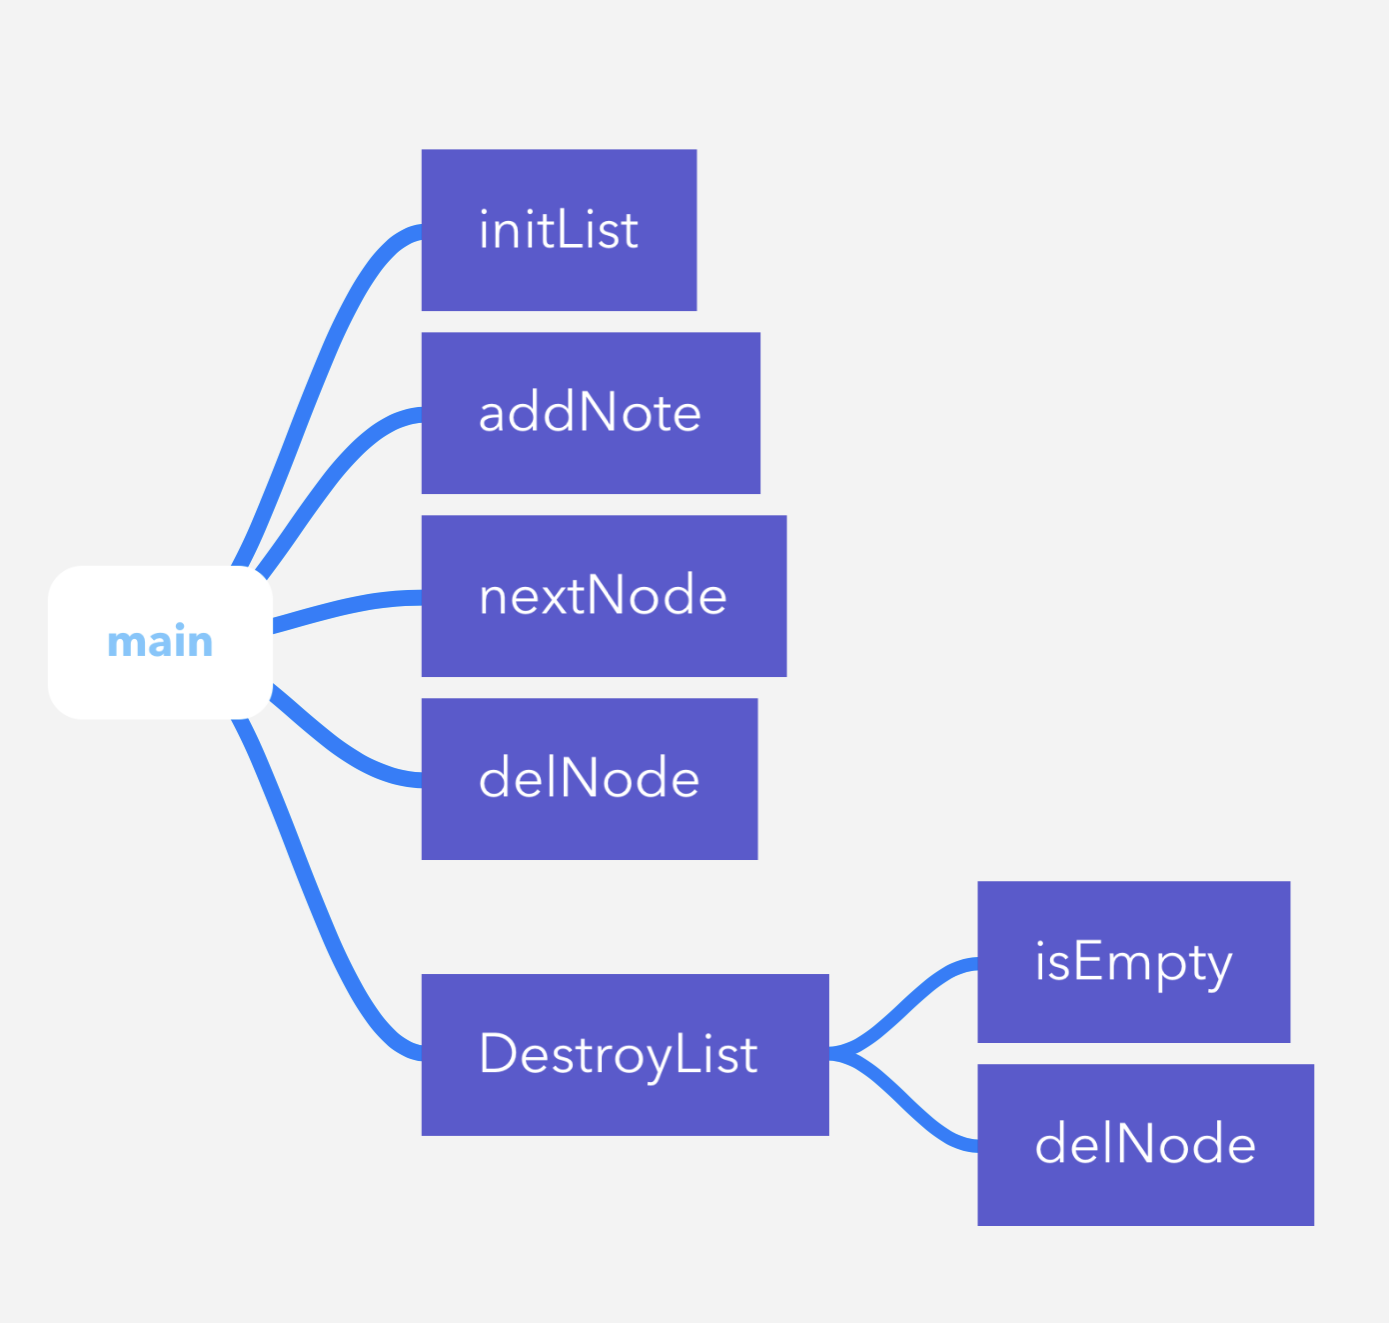
\includegraphics[width=0.4\textwidth]{./Images/pic1.jpg}
    
    \caption{函数的调用关系}
    
\end{figure}

\section{详细设计}

\subsection{链表的实现}

链表设计种基本操作的伪代码算法如下:
\begin{lstlisting}[language={C},
    numbers=left,
    numberstyle=\tiny\menlo,
    basicstyle=\small\menlo]
void initList(List * plist) // 初始化链表
{    
    给*plist分配内存
    if (*plist内存分配失败)
        异常退出
    (*plist)->item <- 0 // 创建空的头结点
    (*plist)->next <- *plist
}

bool isEmpty(const List list) // 判断链表是否为空
{    
    if (List的后继为自身) 返回1
    else 返回0
}

void addNode(List pnode, int item) // 向链表的某个节点后插入一个节点
{    
    创建newNode结点,分配内存
    if (newNode内存分配失败)
        异常退出
    newNode->item <- item
    newNode->next <- pnode->next // 将newNode插入链表内
    pnode->next <- newNode
}

List nextNode(const List pnode) // 找到链表中某一节点的后继
{
    定义nItem为pnode的后继
    if (nItem是头节点) 
        nItem指向它的后继
    返回 nItem
}

void delNode(List pnode) // 删除链表中指定的节点
{
    定义delNode为pnode的后继
    if (delNode是头节点)
        pnode <- delNode, delNode <- delNode->next // pnode和delNode都指向他们的后继
    pnode->next <- delNode->next // 从链表中移除delNode结点
    释放delNode
}

void destroyList(List * plist) // 释放链表空间
{
    while (*plist不为空)
        删除*plist的后继
    释放*plist
    *plist <- NULL
}    
\end{lstlisting}

\subsection{函数的调用关系图}

如2.4所示。

\section{调试分析报告}

\subsection{调试过程中遇到的问题和思考}

初步实现完成后代码即通过样例测试。之后程序多次对边界条件、不合法输入和异常情况进行优化。

\subsection{设计实现的回顾讨论}

由于链表的删除操作实现是删除给定结点的后继,所以$now$指针始终指向当前正在计数元素的前驱。

由于单循环链表中存在一个特殊的头结点,所以另实现一个函数,返回某个结点的后继(跳过头结点)。

删除操作的细节:由于$now$指向正在计数结点的前驱,删除某个结点之后$now$仍然指向原来被删节点的前驱,之后执行$y-1$次寻找后继操作,$now$便指向下一个待删除结点的前驱。

由于主函数对函数的调用足够严密,所以链表的实现没有考虑不符合前件的情况。

由于链表元素均为int类型,所以链表的实现中没有对元素类型进行抽象,并且多次使用赋值运算符更改元素值。

\subsection{算法复杂度分析}

initList,isEmpty,addNode,nextNode,delNode函数的时间复杂度均为$O(1)$。

destroyList函数的时间复杂度为$O(n)$,但是由于主程序调用该函数时链表中一定只有2个结点,故时间复杂度为$O(1)$。

主程序复杂度为$O(n^2)$,整体时间复杂度为$O(n^2)$。

\subsection{改进设想的经验和体会}

\subsubsection{改进1}

在主程序的这一部分:

\begin{lstlisting}[language={C},
    numbers=left,
    numberstyle=\tiny\menlo,
    basicstyle=\small\menlo]
for (int i = 1; i <= n; ++i) // 逐个添加元素
{
    addNode(now, i);
    now = nextNode(now);
}
now = list;
for (int i = 1; i < x; ++i) // 找到第x个元素的前驱
    now = nextNode(now);
\end{lstlisting}

可以另用一个指针变量在向链表逐个添加元素的同时记录第$x-1$个元素的位置,以省去第二个循环。优化后的实现如下:

\begin{lstlisting}[language={C},
    numbers=left,
    numberstyle=\tiny\menlo,
    basicstyle=\small\menlo]
List temp = NULL;
for (int i = 1; i <= n; ++i)
{
    addNode(now, i);
    now = nextNode(now);
    if (i == x - 1) temp = now;
}
now = temp;
\end{lstlisting}

\subsubsection{改进2}

在主程序的这一部分:

\begin{lstlisting}[language={C},
    numbers=left,
    numberstyle=\tiny\menlo,
    basicstyle=\small\menlo]
for (int i = 1; i < n; ++i)
{
    for (int j = 1; j < y; ++j)
        now = nextNode(now);
    delNode(list, now);
}
\end{lstlisting}

对于有$n-i+1$个元素的环,找到当前元素之后的第$y-1$个元素和找到当前元素之后的第$(y-1)\bmod (n-i+1)$个元素并无区别。优化后的实现如下:

\begin{lstlisting}[language={C},
    numbers=left,
    numberstyle=\tiny\menlo,
    basicstyle=\small\menlo]
for (int i = 1; i < n; ++i)
{
    for (int j = 1; j <= (y - 1) % (n - i + 1); ++j)
        now = nextNode(now);
    delNode(list, now);
}
\end{lstlisting}

当$y$比$n$大的时候对时间复杂度有很可观的优化。

\subsubsection{改进3}

约瑟夫问题有时间复杂度为$O(n)$的递归解法,现论述如下:

假设对于有$n$个元素的环,序号为0至$n-1$,以序号为0的元素为起点,删去第$y$个元素,即序号为$y-1$的元素,之后进行下一次删除。

而根据题意,下一次删除应该从被删除元素的下一个元素开始计数,所以可以将整体序号减去$y$再对$n$取余数,得到新的序号,范围是0至$n-2$,然后再以0为起点重复删除操作。

最后一次删除和序号变化之后,剩余一个序号为0的元素。可以根据上述操作的逆过程推出这个元素在初始状态下的序号。

由于题目规定了起点的序号为$x$,所以还要再进行一次类似的整体序号位移,另外题目中序号为1至$n$,给求得答案$+1$得到题目要求的答案。

该解法的实现如下:

\begin{lstlisting}[language={C},
    numbers=left,
    numberstyle=\tiny\menlo,
    basicstyle=\small\menlo]
#include <stdio.h>

int main()
{
    int n, x, y;
    scanf("%d%d%d", &n, &x, &y);
    int ans = 0;
    for (int i = 2; i <= n; ++i)
        ans = (ans + y) % i;
    printf("%d\n", (ans + x - 1) % n + 1);
    return 0;
}
\end{lstlisting}

这个程序(main1.c)被用于测试环节,用来验证原解法的正确性。

\section{用户使用说明}

使用gcc编译生成可执行文件。

\begin{lstlisting}[language={bash},
    basicstyle=\small\menlo]
gcc -o main -std=c11 main.c list.c
\end{lstlisting}

执行可执行文件:

\begin{lstlisting}[language={bash},
    basicstyle=\small\menlo]
./main
\end{lstlisting}

在Windows cmd下:

\begin{lstlisting}[language={bash},
    basicstyle=\small\menlo]
main
\end{lstlisting}

之后通过标准输入输入数据,输入格式参考1.2节的输入描述,结果通过标准输出返回。如果输入合法并且程序正常运行结束,主函数返回值为0。

\section{测试结果}

测试环节分为四个步骤。

\subsection{测试第一部分}

对1.4节给出的样例进行测试。

\subsection{测试第二部分}

在delNode函数中添加输出语句,输出每一轮计数时的第$y$个元素,输入小样例,将输出与手动模拟结果比对。

【输入】

\begin{lstlisting}[language={bash},
    basicstyle=\small\menlo]
10 1 3
\end{lstlisting}

【输出】

\begin{lstlisting}[language={bash},
    basicstyle=\small\menlo]
3
6
9
2
7
1
8
5
10
No
4
4
\end{lstlisting}

此样例中环中删除的元素依次为3,6,9,2,7,1,8,5,10,4,与模拟结果相符。

\subsection{测试第三部分}

测试非法输入和边界条件。

【输入】

\begin{lstlisting}[language={bash},
    basicstyle=\small\menlo]
5 -1 2
\end{lstlisting}

【输出】

\begin{lstlisting}[language={bash},
    basicstyle=\small\menlo]
Please check your input.
\end{lstlisting}

【输入】

\begin{lstlisting}[language={bash},
    basicstyle=\small\menlo]
5 2 -1
\end{lstlisting}

【输出】

\begin{lstlisting}[language={bash},
    basicstyle=\small\menlo]
Please check your input.
\end{lstlisting}

【输入】

\begin{lstlisting}[language={bash},
    basicstyle=\small\menlo]
1000000 256 512
\end{lstlisting}

【输出】

\begin{lstlisting}[language={bash},
    basicstyle=\small\menlo]
Please check your input.
\end{lstlisting}

【输入】

\begin{lstlisting}[language={bash},
    basicstyle=\small\menlo]
10000 5723 4627
\end{lstlisting}

【输出】

\begin{lstlisting}[language={bash},
    basicstyle=\small\menlo]
No
5180
\end{lstlisting}

\subsection{测试第四部分}

将原解法与4.4.3中的改进解法比对。

测试在macOS\ Catalina\ 10.15.6下进行。

在$n<=10$,$n<=1000$,$n<=10000$的范围下分别随机生成1000组测试数据,分别传入main和main1,并且比对两程序的输出。

3000组数据中两程序的输出均相同。

数据生成程序(data.cpp)如下:

\begin{lstlisting}[language={C++},
    numbers=left,
    numberstyle=\tiny\menlo,
    basicstyle=\small\menlo]
#include <bits/stdc++.h>
using namespace std;

const int LIMIT = 98;

int main()
{
    srand(time(0));
    int n, x, y;
    n = rand() % LIMIT + 2;
    x = rand() % n + 1;
    y = rand() % (n * 3) + 2;
    printf("%d %d %d\n", n, x, y);
    return 0;
}
\end{lstlisting}

比对脚本(chk.cpp)如下:

\begin{lstlisting}[language={C++},
    numbers=left,
    numberstyle=\tiny\menlo,
    basicstyle=\small\menlo]
#include <bits/stdc++.h>
using namespace std;
int main()
{
    int T = 1000;
    while (T--)
    {
        system("./data >in.in");
        system("./main <in.in >out.out");
        system("./main1 <in.in >out1.out");
        if (system("diff out.out out1.out"))
            break;
        puts("Correct");
    }
    return 0;
}
\end{lstlisting}

\section{可视化}

\subsection{过程可视化}

使用JavaScript实现过程可视化。

\subsubsection{实现细节}

程序运行后,读取用户输入的$n, x, y$参数,进行参数类型转换。通过  document.getElementById 获取画布。创建双链表。以上三者存放在 然后存放到 simulator 的 store 成员中。

通过$2\pi$均分获取角度差,通过画布的长宽确定中心点。一中心点为圆心,通过 center.x + radius * Math.cos(deltaDegree * i); 和 center.y + radius * Math.sin(deltaDegree * i); 分别计算各个圆的位置。使用 20 作为半径绘制圆。分别在个个圆上绘制文本。通过定时器模拟人员活动,每 100 毫秒执行。根据存活状况更新各个圆的颜色,通过 currentNode 和 flag 局部变量存放当前节点和跳过人数。当剩余一个人时停止计时。

使用JavaScript实现双向链表模拟环中元素的关系。

\subsubsection{用户使用说明}

使用现代浏览器打开Animation/index.html,根据提示输入$n, x, y$,要求输入合法且$1 < n < 40$,之后页面展示一段动画,内容为约瑟夫问题的过程。

\subsubsection{示例}

见图2。

\begin{figure}[htbp]
    
    \centering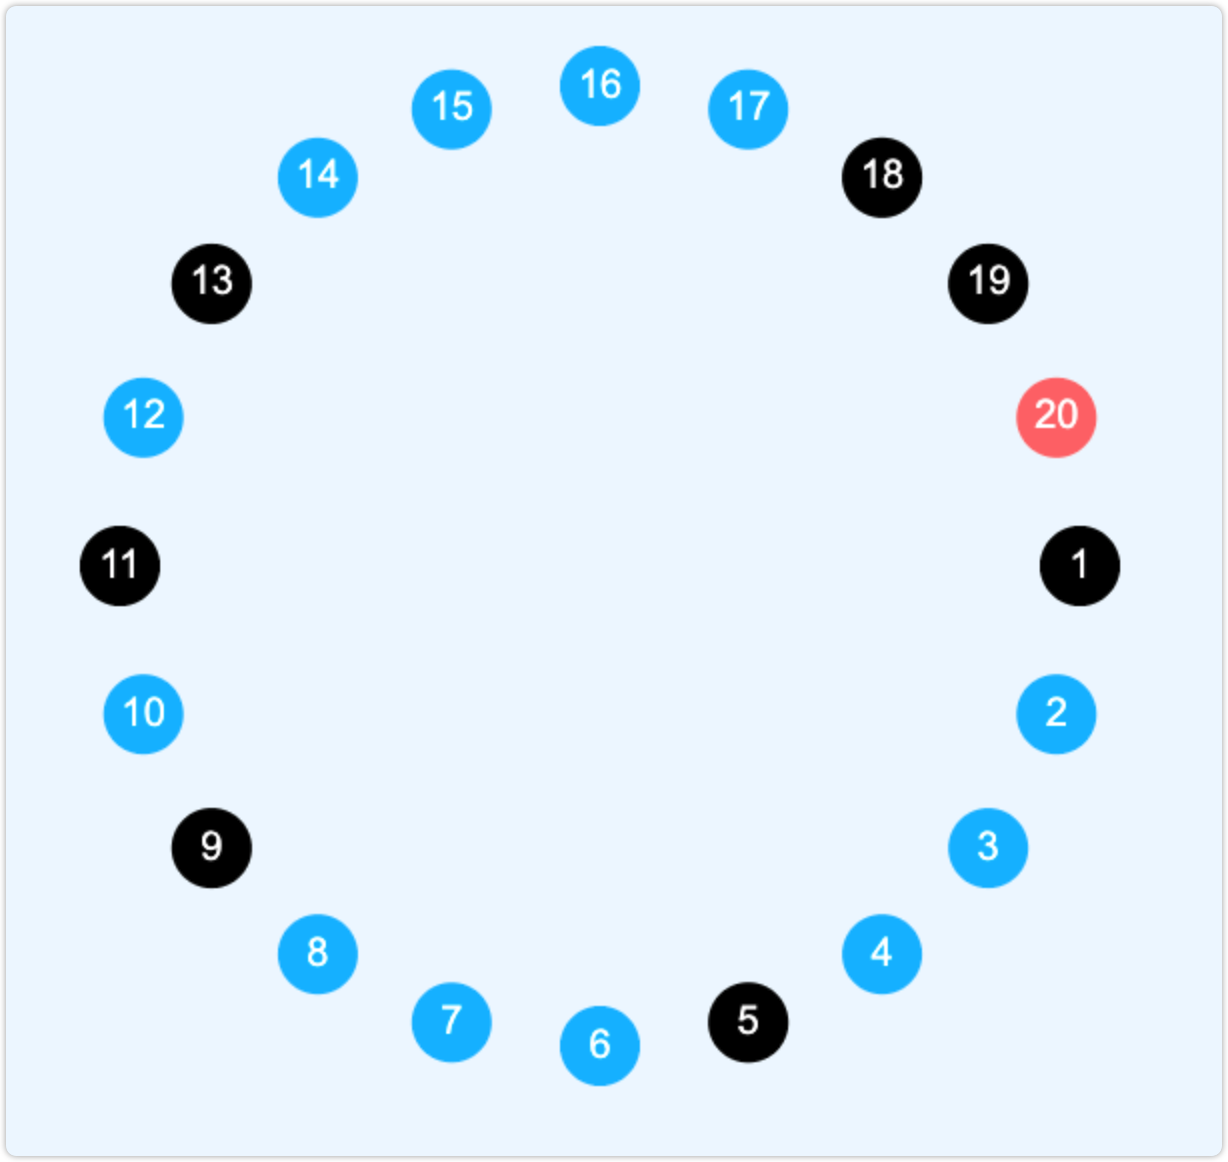
\includegraphics[width=0.6\textwidth]{./Images/Animation.png}
    
    \caption{过程可视化示例}
    
\end{figure}

\subsection{结果可视化}

使用JavaScript实现结果可视化。

\subsubsection{实现细节}

程序运行后,读取用户输入的$n$参数,之后利用使用JavaScript实现的4.4.3节改进算法计算$1 \leq x\leq n,1\leq y\leq n$中的所有解,导出为点集。

使用Highcharts库绘制3D散点图,展示所求出的点集。

\subsubsection{用户使用说明}

使用现代浏览器打开Scatter/index.html,根据提示输入n,要求$1 < n <= 25$,之后页面展示一张散点图。

拖动该散点图可以旋转,将鼠标指针放到某个点上可以看到该点的值。

\subsubsection{示例}

见图3。

\begin{figure}[htbp]
    
    \centering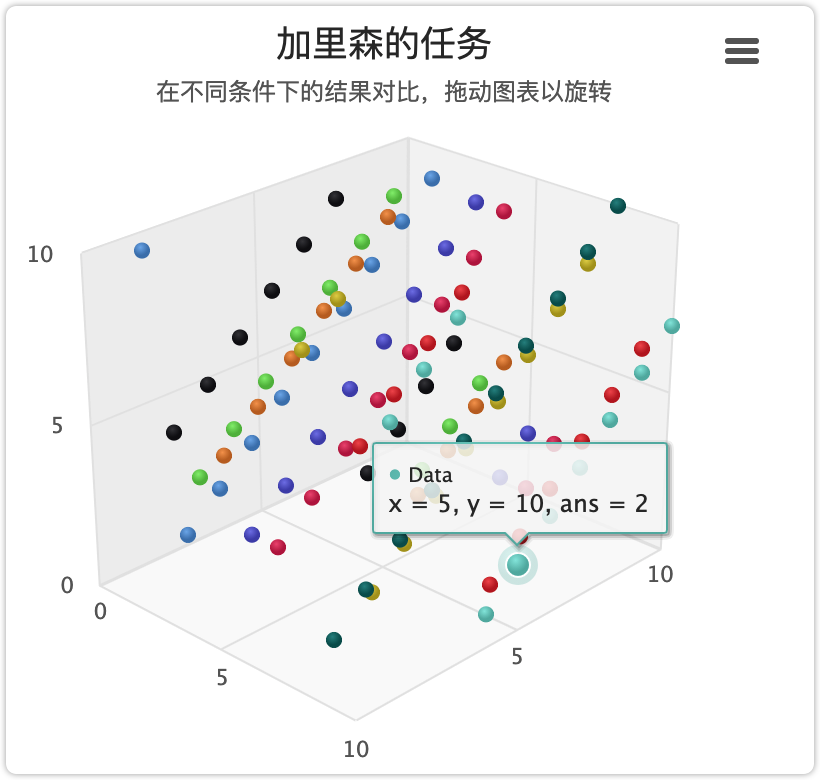
\includegraphics[width=0.6\textwidth]{./Images/Scatter.png}
    
    \caption{结果可视化示例}
    
\end{figure}

\subsubsection{结论}

可以明显地看出,当$n$一定,$y$一定时,由于$x$增加1时$ans$也对应地增加1,所以这些点分布在一条直线上。

\end{document}
